\documentclass{beamer}
\usepackage[utf8]{inputenc}
%\usepackage{AlDraTex}
\usepackage{alltt}
\usepackage{amsthm}
\usepackage[english,russian]{babel}
\usepackage{graphics}
\usepackage{subfigure}
\usepackage{color}
\usepackage{colordvi}
%\usepackage{tikz}
\definecolor{royalblue}{RGB}{65,105,225}
\definecolor{stateblue}{RGB}{106,90,205}
\usepackage{cmap}
\usetheme{Singapore}
\newcommand{\pval}{\text{\textit{p-value}}}
\renewcommand*{\thesubfigure}{}
%\useoutertheme{infolines}
%\usetheme{Darmstadt}
%\usecolortheme{seahorse} 
\usepackage{url}
%\usepackage{cite}
%\usepackage[square]{natbib}
%\newcommand{\newblock}{}
%\renewcommand{\bibsection}{\subsubsection*{\bibname } }\setlength{\unitlength}{1in}
\newcounter{story}
\graphicspath{{./img/}}
\title{p-values: what do they mean, how to calculate them, how do they behave and what to do if there are a lot of them}
\date{2011-2020}
\author[A Favorov]{
Alexander Favorov
}
\begin{document}
\begin{frame}
	\titlepage
\end{frame}
%\section{Outline}
%\begin{frame}
%	\frametitle{Outline}
%	\tableofcontents
%\end{frame}
\addtocounter{story}{1}
\section{Story \arabic{story}\ :\ p-values}
	\begin{frame}
		\begin{center}
			\huge{Story \arabic{story}\ :\ p-values}
		\end{center}
	\end{frame}
	\begin{frame}
		\frametitle{Null hypothesis and p-value}
		Philosophical concept: everything is bad!
		
		Null hypothesis: Our signal is noise. 
			
		\begin{center}
			A model for noise $\Rightarrow$ probabilistic decsription of what happens.
			
			\vskip .1in

			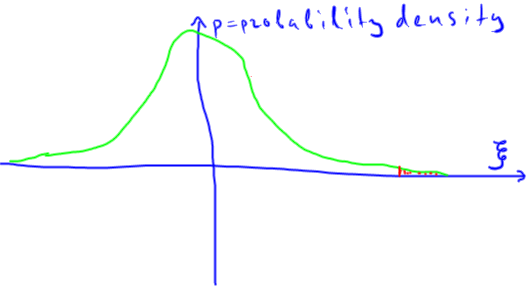
\includegraphics[scale=.4]{p-value}

			$\pval=\int_{\xi_{obs}}^{\infty}p\left( \xi \right) d\xi = 1-\text{cdf}\left( \xi_{obs} \right) $
		\end{center}
	\end{frame}
	\begin{frame}
		\frametitle{Two -sided p-value}
		Just to mention
		\begin{center}

			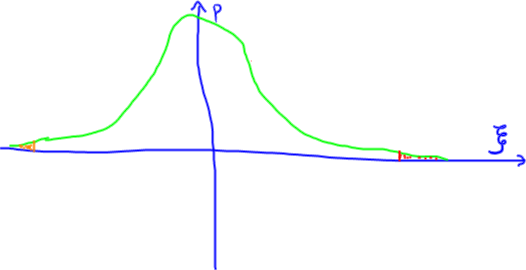
\includegraphics[scale=.4]{p-value-2-tail}

		\end{center}
	\end{frame}
	
	\begin{frame}
		\frametitle{P-values \& Bayesian paradigm}
		\begin{center}

			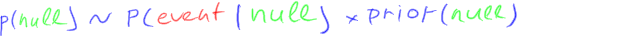
\includegraphics[scale=.4]{bayes_p_val}

			\vskip .1in

		p-value is a conditional probability ... \textcolor{red}{what of???}

		\end{center}
			\vskip .1in

		Cons: it is a probability of a tail

		Cons: no confidence interval

			\vskip .1in

		Pros: it is a probability of a tail.
		
		\begin{itemize}	
			
			\item Normalization.

			\item We are not to know a signal model.

		\end{itemize}	

	\end{frame}
	
	\begin{frame}

		\frametitle{\small{AMERICAN STATISTICAL ASSOCIATION RELEASES STATEMENT ON
STATISTICAL SIGNIFICANCE AND P-VALUES\\March 7, 2016 }}
		\begin{enumerate}	
				\item P-values can indicate how incompatible the data are with a specified statistical model.
				\item P-values do not measure the probability that the studied hypothesis is true, or the
probability that the data were produced by random chance alone.
\item Scientific conclusions and business or policy decisions should not be based only on
whether a p-value passes a specific threshold.
\item Proper inference requires full reporting and transparency.
\item A p-value, or statistical significance, does not measure the size of an effect or the
importance of a result.
\item By itself, a p-value does not provide a good measure of evidence regarding a model or
hypothesis.
		\end{enumerate}	
	
	
	\end{frame}

	\begin{frame}
		\frametitle{Threshold}
		\begin{itemize}	
			\item Traditional: 0.05
			\item Redefine statistical significance. Daniel J. Benjamin \textit{et al}, Nature Human Behaviour, 2017
			\item More confident: 0.005
			\item Changing the significance threshold is a distraction from the real solution, which is to replace null hypothesis significance testing (and bright-line thresholds) with more focus on effect sizes and confidence intervals, treating the P value as a continuous measure, and/or a Bayesian method.
		\end{itemize}	
	\end{frame}
	
	\begin{frame}
		\frametitle{How do people calculate it?}
		\begin{itemize}	
		\item Parametric tests

			\vskip .1in

		\item Nonparametric tests

			\vskip .1in

		\item Combinatorial (Fisher)

			\vskip .1in

		\item Permutation

		\end{itemize}	
	\end{frame}

	%\renewcommand*{\thesubfigure}{}
	\begin{frame}
	\frametitle{Exact Fisher test (1922)}
		\begin{center}
		\begin{figure}[ht]
			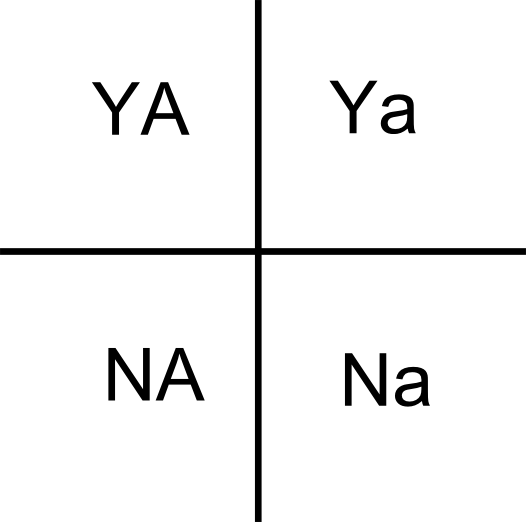
\includegraphics[scale=0.4]{fisher-contig}
		\end{figure}
		\end{center}
	Exact Fisher test: association. Null-hypothesis: $Y/N$ is not associated with $A/a$. Let's denote the whole population as $M$. We consider only those contigency tables that has the same $M$, $Y$, $N$, $A$ and $a$ populations.

	\vspace{.2in}
	\begin{figure}[ht]
		\subfigure[....]{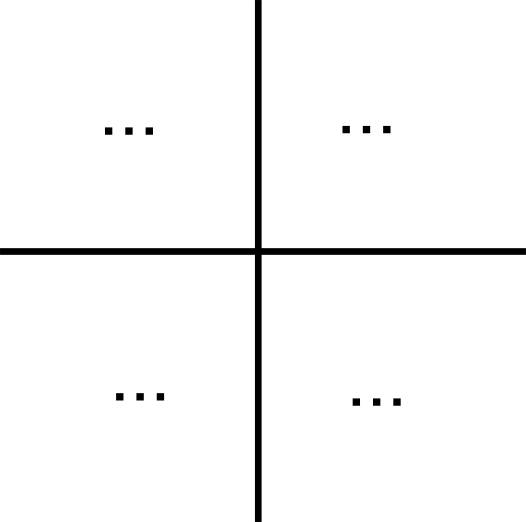
\includegraphics[scale=0.3]{fisher-etc}}
		\subfigure[Previous]{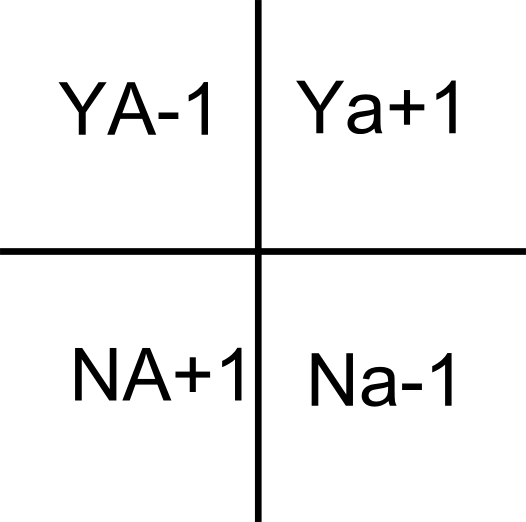
\includegraphics[scale=0.3]{fisher-contig--}}
		\subfigure[\bf{Our}]{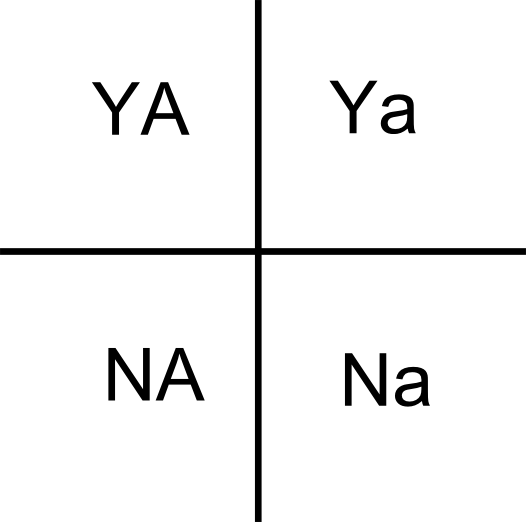
\includegraphics[scale=0.3]{fisher-contig}}
		\subfigure[Next]{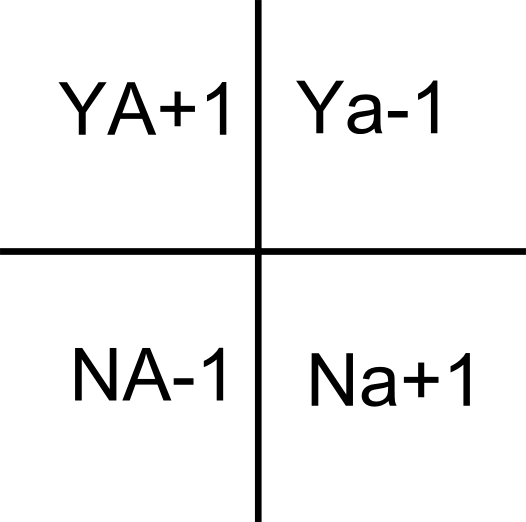
\includegraphics[scale=0.3]{fisher-contig++}}
		\subfigure[....]{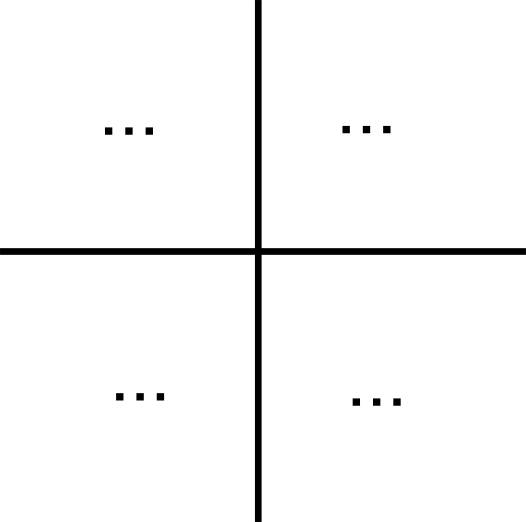
\includegraphics[scale=0.3]{fisher-etc}}
		\begin{center}
	Parametrized family of contigency table classes.
		\end{center}
	\end{figure}
	\end{frame}
	%\renewcommand*{\thesubfigure}{(\alph{subfigure})}

	\begin{frame}
	\frametitle{Exact Fisher test: calculation}
		\begin{center}
		\begin{figure}[ht]
			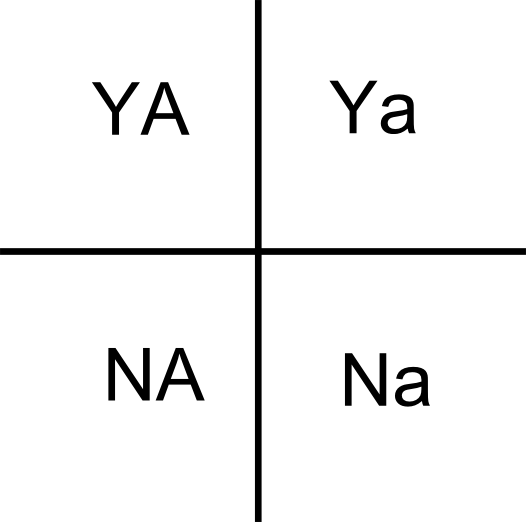
\includegraphics[scale=0.2]{fisher-contig}
		\end{figure}
		\end{center}

	Population of each class of tables is: 
	$$\displaystyle P(YA)=\binom{A}{YA}\binom{a}{Ya}=\frac{A!a!}{YA!Ya!NA!Na!}$$
	All the tables has different scheme of $A/a$ ascribing to cases and to controls. 
	We do not need to sum it for normalisation, the overall population is just $\displaystyle\sum_{YA}{P(YA)}=\binom{M}{Y}$.

	The $\pval$ of our table is sum of normalized populations of one of the tails of the parametrized family, starting from our.
	\end{frame}

	\begin{frame}
	\frametitle{Exact Fisher test: three magic things}
	\begin{itemize}
		\item A parameter that grows monotonously with the association.
		\item Combinatorial calculations for null-hypothesis.
		\item Simple normalization (not too critical now).
	\end{itemize}
	\end{frame}


	\begin{frame}
		\frametitle{Permutation}
		\begin{center}
			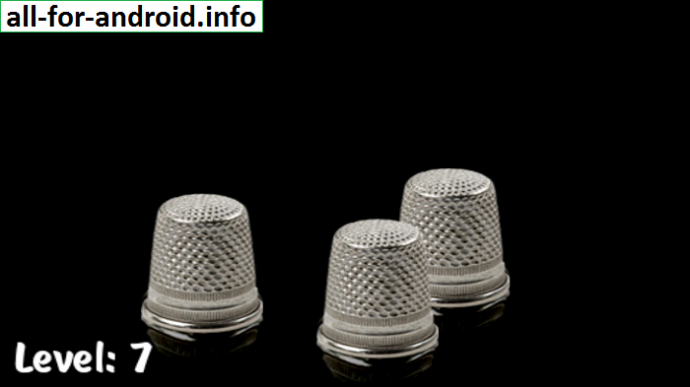
\includegraphics[scale=0.2]{naperstke}

			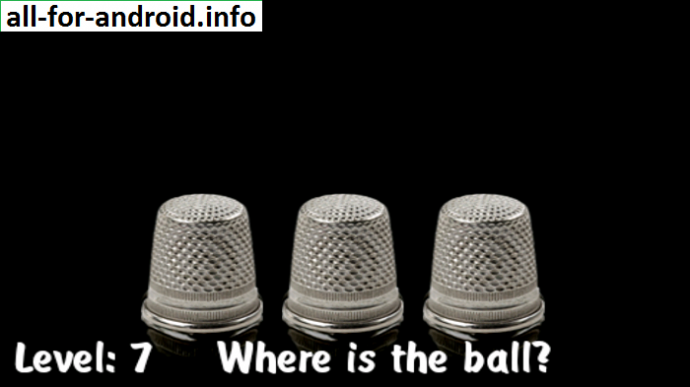
\includegraphics[scale=0.2]{naperstke-script}

			\vskip .1in

			Null model is generated from the data by removing \\ any sense that we are looking for.
		\end{center}
	\end{frame}

	\begin{frame}
		\frametitle{P-values are distributed uniformly!}
		\begin{center}
			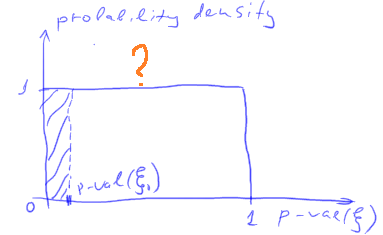
\includegraphics[scale=0.6]{p_val_is_flat_by_def_picture}
		\textcolor{violet}{$$ P\left(\pval\left(\xi\right) \leq \pval\left(\xi_0\right)\right)=\pval\left(\xi_0\right)$$}
		The formula is just the definition of p-value and the fact that $\pval\left(\xi\right)$ changes monotonously with $\xi$.

		$\pval\left(\xi_0\right)$ is distributed as 1x1 box, i.e. uniformly.
		\end{center}
	\end{frame}

	\begin{frame}
		\frametitle{Density of function of a random variable}
		$\xi$ is a r.v.

		$\rho\left(\xi\right)$ is its probability density
		
		$g\left(\xi\right)$ is a function of $\xi$ 
		
		$\rho\left(g\left(\xi\right)\right)$ is $g$'s probability density
		
		\vskip .1in
		\begin{center}
			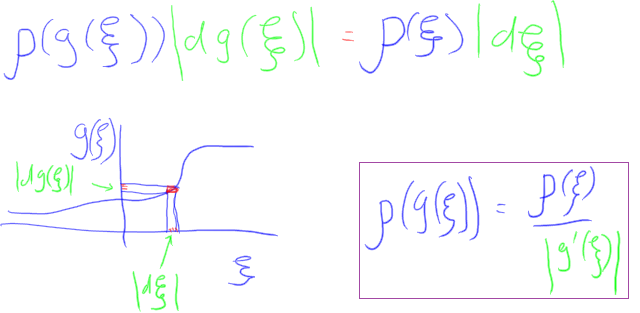
\includegraphics[scale=0.4]{density_of_function}
		\end{center}
	\end{frame}
	\begin{frame}
		\frametitle{P-value is distributed uniformly, again.}
		\begin{center}
			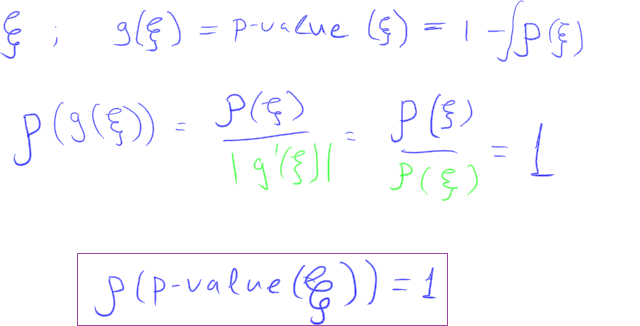
\includegraphics[scale=0.6]{p_val_is_flat}
		\end{center}
	\end{frame}
\addtocounter{story}{1}
\section{Story \arabic{story}\ :\ Multiple hypothesis correction}
	\begin{frame}
		\begin{center}
			\huge{Story \arabic{story}\ :\ Multiple hypothesis correction}
		\end{center}
	\end{frame}

	\begin{frame}
		\frametitle{Multiple hypohtesis. Bonferroni correction.}
		\vskip .1in
		Suppose we have a good (e.g. $0.001$) p-value.\\
		But it is the best result of N (say, 100) experiments.\\ 
		What does the p-value actually mean?
		$$0 \leq p_1 \leq p_2 \leq p_3 \leq p_4 \leq \ldots \leq p_N$$
		For one test:\textcolor{violet}{$$ P\left(\pval\left(\xi\right) \leq p\right)=p)$$}
		
		Bonferroni: for  $N$ tests: Boole's inequality:
		$$ \pval_{corr}=P\left(\text{any } \pval\left(\xi\right) \leq p \right)=N p$$

		Or, more precisely, 
		$$ \pval_{corr}=1-\left(1-p\right)^N \approx Np \text{ if } N p \ll 1$$
		\begin{center}
		\end{center}
	\end{frame}

	\begin{frame}
		\frametitle{Bonferroni correction is FWER}
		\begin{itemize}	
			\item Supposes all the p-values are independent.
			\item Requires that there is no noise (in the sense of a single test) in the whole good (rejected null) set. Clever word: FWER Famile-Wise Error Rate.
		\end{itemize}
\vskip .6in
\small{Bland, J. M. and D. G. Altman (1995). Multiple significance tests: the Bonferroni method.
BMJ (Clinical Research Ed.) 310 (6973), 170. PMID: 7833759.}
	\end{frame}
	
	\begin{frame}
		\frametitle{Holm-Bonferroni: FWER revisited}
		\begin{center}
		$$0 \leq p_1 \leq p_2 \leq p_3 \leq p_4 \leq \ldots \leq p_N$$
		
		We want $FWER \leq \alpha$.
		
		\vskip .1in
		$\text{min }i: {p_i} > \displaystyle\frac{\alpha}{N-i+1}$ is the first non-rejected null
		\end{center}

		Indeed, $P \left( \exists \text{real null}:p<\displaystyle\frac{\alpha}{m_0} \right) <= m_0 \displaystyle\frac{\alpha}{m_0}=\alpha$, 
		
		where $m_0$ is number of real nulls (unknown).
		
		\vskip .1in
		And, if $ p>=\displaystyle\frac{\alpha}{m_0} $ for all real nulls, 
		we cannot jump over a real null, $N-i+1$ includes $m_0$ real nulls.	
		\vskip .2in
		Holm, S. (1979). "A simple sequentially rejective multiple test procedure". Scandinavian Journal of Statistics. 6 (2): 65–70. JSTOR 4615733. MR 0538597

	\end{frame}

	\begin{frame}
		\frametitle{Westfall-Young permutation method}
			\begin{minipage}[0.2\textheight]{\textwidth}
			\begin{columns}[T]
			\begin{column}{0.15\textwidth}
				
\includegraphics[width=\textwidth]{djinn}
			\end{column}
			\begin{column}{0.85\textwidth}
				$$0 \leq p_1 \leq p_2 \leq p_3 \leq p_4 \leq \ldots \leq p_N$$
				We want to have corrected (FWER) p-values, and we do not want to worry about dependencies!
			\end{column}
			\end{columns}
			\end{minipage}
		\begin{center}
			We permute the data that underlies the p-values M times so that the structure is maintaned while the sense (if it was) disappears. 
				\tiny{\begin{align*}
				&0   & \leq &   p_1^1  & \leq &  p_2^1  & \leq &  p_3^1  & \leq &  p_4^1  & \leq &  \ldots  & \leq &  p_N^1 \\
				&0   & \leq &   p_1^2  & \leq &  p_2^2  & \leq &  p_3^2  & \leq &  p_4^2  & \leq &  \ldots  & \leq &  p_N^2 \\
				&0   & \leq &   p_1^3  & \leq &  p_2^3  & \leq &  p_3^3  & \leq &  p_4^3  & \leq &  \ldots  & \leq &  p_N^3 \\
				& \ldots &&  \ldots && \ldots && \ldots && \ldots && \ldots && \ldots \\
				&0   & \leq &   p_1^M  & \leq &  p_2^M  & \leq &  p_3^M  & \leq &  p_4^M  & \leq &  \ldots  & \leq &  p_N^M
				\end{align*}}\normalsize{}
		$p_i^{WY} = \displaystyle\frac{\#k: p_i^k \leq p_i }{M}$. It is SLOW!
		\end{center}
		%\vskip .6in
		\small{Westfall, P. H. and S. S. Young (1993). Resampling-based multiple testing. John Wiley and Sons.}
	\end{frame}

\addtocounter{story}{1}
\section{Story \arabic{story}\ :\ Error rate control}
	\begin{frame}
		\begin{center}
			\huge{Story \arabic{story}\ :\ Error rate control}
		\end{center}
	\end{frame}

	\begin{frame}
		\frametitle{Recognition tasks: How to tell set 1 from set 2?}
		\begin{center}
			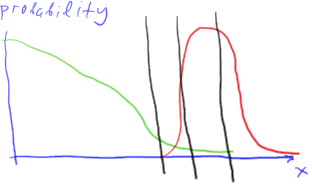
\includegraphics[scale=0.6]{discriminate}


			Noise (не конфетки) is green, \\ signal (конфетки) is red. Threshold?
		\end{center}
		\begin{itemize}
		\item Type I error: noise is misinterpreted as signal. \\ False positive.
		\item Type II error: signal is misinterpreted as noise. \\ 1-power(signal). False negative.
		\end{itemize}
	\end{frame}

	\begin{frame}
		\frametitle{FDR}
		\begin{center}
			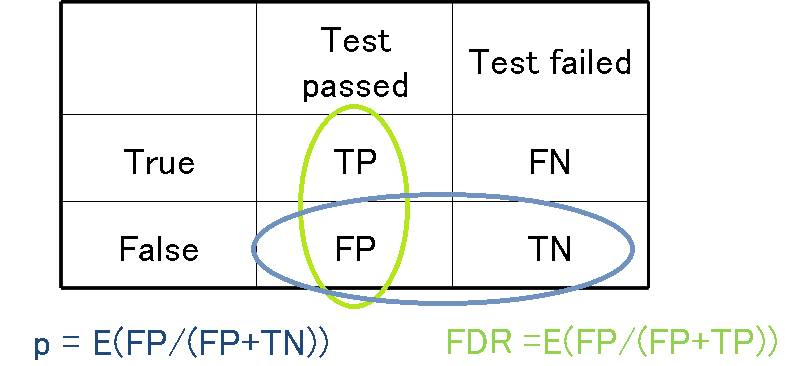
\includegraphics[scale=0.5]{FDR}
		\end{center}
		Only noise model was necessary to evaluate p-value. To know FDR, we need some propositions about the signal.
	\end{frame}

	\begin{frame}
		\frametitle{Error rate control}
		$$0 \leq p_1 \leq p_2 \leq p_3 \leq p_4 \leq \ldots \leq p_N$$

		Let's try to find $i$ splitting our set to noise and signal so that we like it.

		\begin{itemize}
		\item We want the probability to get any (at least one) noise point below $i$ to be $\alpha$. FWER. Family is what we took as signals. So, we choose $i$ so that Bonferroni or WY-corrected $\pval_{corr}\left(i\right)\leq \alpha$. Type I error is low, but the Type II is high.  
		\item FDR : False Discovery Rate
		\end{itemize}
	\end{frame}

	\begin{frame}
		\frametitle{Benjamini, Hochberg}
		\begin{center}
		$$0 \leq p_1 \leq p_2 \leq p_3 \leq p_4 \leq \ldots \leq p_N$$
		
		We want $FDR \leq \alpha$.
		\end{center}
		
		$$\text{max }i: \frac{Np_i}{i} \leq \alpha$$

		Indeed, we have $i$ items that passed our test and we estimate the number of FP's as $Np_i$. The estimation assumes independency, it is a close relative of Bonferroni.
		\vskip .2in
		Benjamini, Y. and Y. Hochberg (1995). Controlling the false discovery rate: A practical
		and powerful approach to multiple testing. Journal of the Royal Statistical Society. 
		Series B (Methodological) 57 (1), 289-300.

	\end{frame}

	\begin{frame}
		\frametitle{Storey, Tibshirani}
		\begin{center}
			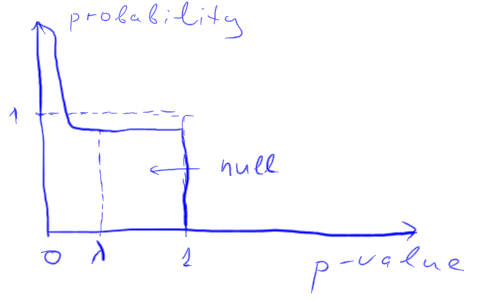
\includegraphics[scale=0.4]{Storey}
		\end{center}
	
	
	This is an observed distribution that is converted to p-values using a noise model. If the noise model is appropriate, the correponding noise part is a rectangular area.

	\vskip .1in
	Storey, J. D. and R. Tibshirani (2003, August). Statistical significance for genomewide
	studies. PNAS 100 (16), 9440-9445. PMID: 12883005.
	\end{frame}

	\begin{frame}
		\frametitle{Rank-based threshold}
			$S_1 \geq S_2 \geq S_3 \geq \ldots \geq S_N$ ; $p(S_i)=P(S<S_i)$ for null (noise) S.
			$p(S_1) \leq p(S_2) \leq p(S_3) \leq \ldots \leq p(S_N)$.

	\vskip .1in
			We want to choose $i$ that splits the set into signal and noise. 
			
	\vskip .1in
			We can imagine our signal as a Bernoulli process with success probability $p(S_i)$ and we got at least $i$ successes from $N$ trials. Let's choose $i$ that minimise this probability:

			$$i=argmin\left(\sum_{k=1}^{i}\binom{N}{k}p(S_i)^k\left(1-p(S_i)\right)^{N-k}\right)$$
	\vskip .2in
	O.V. Kalinina, P.S. Novichkov, A.A. Mironov, M.S. Gelfand, and A.B. Rakhmaninova. NAR 2004 July 1; 32

	\end{frame}

%\addtocounter{story}{1}
%\section{Story \arabic{story}\ :\ Random variable generation}
%	\begin{frame}
%		\begin{center}
%			\huge{Story \arabic{story}\ :\ Random variable generation}
%		\end{center}
%	\end{frame}

\section{Conclusions}

\begin{frame}
\frametitle{Conclusions}
\begin{center}
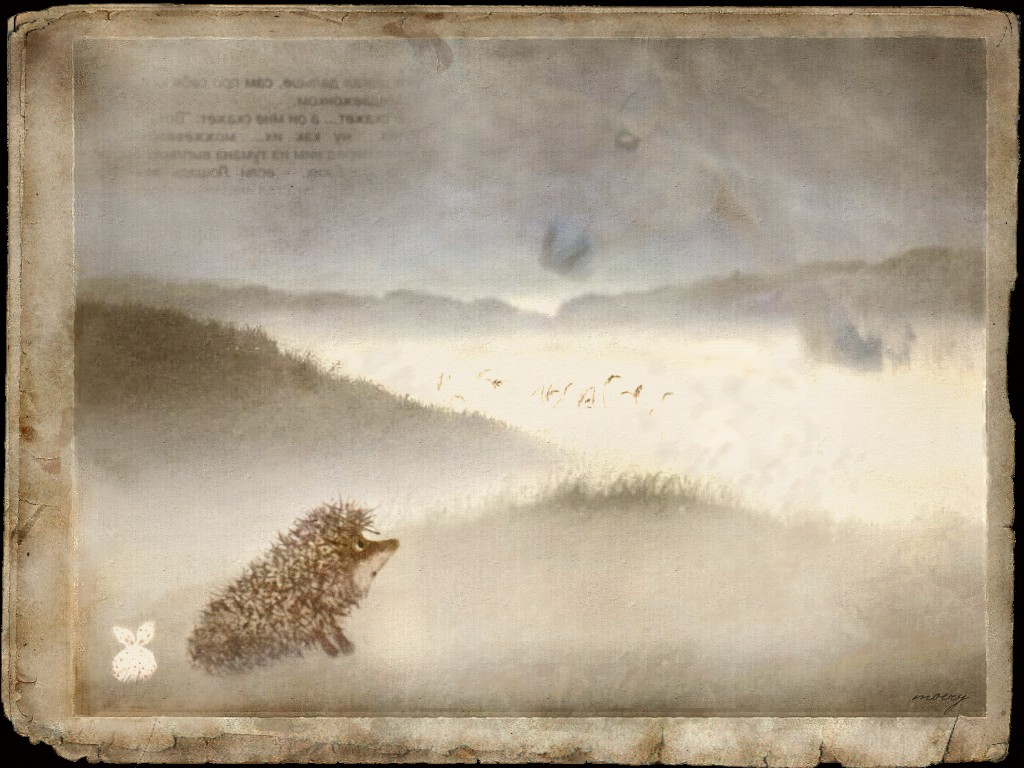
\includegraphics[scale=0.25]{yozhik}
\end{center}
\end{frame}

%\section*{fin}
\bibliographystyle{natbib}
\bibliography{p-value}

\end{document}
 

